\chapter{How Balance Leads to Productivity}

This lecture is not a formal mathematical lecture in the usual sense, but it is built around a real constraint: time is finite. The speaker begins with the fixed size of a day, admits that entrepreneurial life sometimes requires temporary imbalance, and then asks how we design the ordinary majority of life so that work, recovery, family, and self-direction can all survive. These notes follow the School of Hard Knocks source material, curated by LazyingArt LLC, and treat the transcript as the primary evidence.

\section{The Twenty-Four-Hour Constraint}

The lecture opens with the simplest possible budget constraint. We have only so much time in a day, and every responsibility must live inside that boundary. Written as bookkeeping, the constraint is

\begin{equation}
T_{\mathrm{day}} = 24\ \mathrm{hours}.
\end{equation}

The opening question is therefore not vague. It is an allocation problem. If work, responsibilities, self-care, friends, and family all require time, then a balanced life cannot mean doing everything without cost. It means deciding what receives time and when.

A useful first model is

\begin{equation}
T_{\mathrm{day}}
=
T_{\mathrm{work}}
+
T_{\mathrm{responsibilities}}
+
T_{\mathrm{self}}
+
T_{\mathrm{family/friends}}
+
T_{\mathrm{recovery}}.
\end{equation}

This equation is not on a blackboard in the source video; it is a clean reconstruction of the speaker's practical claim. Balance means making time for the things one has to do and also for the things one wants to do.

\subsection{Question \& Answer}

\paragraph{Question.}
If the day has only twenty-four hours, how do we handle responsibilities while still making time for ourselves, friends, and family?

\paragraph{Answer.}
We stop treating balance as a feeling and treat it as a designed allocation. Some time must go to obligations; some time must be protected for the rest of life. The lecture's first point is that balance begins when we see the day as finite.

\section{Necessary Imbalance}

The speaker immediately adds a caveat. Balance is not a rule that every day must satisfy. There are seasons when imbalance is real and sometimes unavoidable.

The entrepreneurial example is concrete: if a project has the potential to change one's life and the lives of others, the workday may sometimes become

\begin{equation}
T_{\mathrm{work}} \approx 16\ \mathrm{hours}.
\end{equation}

Those are not balanced days. The lecture also gives the example of a parent with a newborn: the parent is not making the schedule; the baby is. The point is not to glorify imbalance, but to locate it. Imbalance may be locally rational during exceptional periods, but it should not quietly become the default pattern.

The speaker then narrows the target. The practical methods in the lecture apply to the ordinary majority of life, approximately

\begin{equation}
0.80 \leq f_{\mathrm{ordinary}} \leq 0.85.
\end{equation}

This is not a measured statistic; it is the speaker's working estimate. The important distinction is between unavoidable exceptional seasons and the larger portion of life where we can actually implement systems.

\section{Why Balance Matters}

The next movement in the lecture asks why balance matters at all. The first answer is mental health. A person can keep working for a while without reflection, but eventually the cost appears in stress, relationships, motivation, and the quality of work itself.

\subsection{Question \& Answer}

\paragraph{Question.}
How do we know whether work-life balance has become unhealthy?

\paragraph{Answer.}
The lecture's diagnostic is reflective rather than technical: pause and ask what is actually causing stress, and ask what is being prioritized right now. In symbols, we can write this as a simple state check:

\begin{equation}
\mathrm{State}
=
\left(
\mathrm{Stressors},
\mathrm{Priorities},
\mathrm{Direction}
\right).
\end{equation}

The point of the notation is only to make the pause explicit. We inspect the current state before trying to optimize it.

This is one of the lecture's central rhythms: do not rush directly to productivity tactics. First ask whether the way we are living and working is actually working.

\section{Burnout As Lost Capacity}

The second reason balance matters is burnout. The transcript defines burnout plainly: it is the state where one lacks the strength and the desire to continue working on the thing at hand. The speaker describes it as detachment, low imagination, low creativity, and no desire to work.

For entrepreneurship, that matters because the damaged object is not only mood. It is productive capacity. If we let \(C\) denote working capacity in a broad practical sense, then the lecture's mechanism can be summarized as

\begin{equation}
\mathrm{Lack\ of\ balance}
\longrightarrow
\mathrm{burnout}
\longrightarrow
C \downarrow .
\end{equation}

This is not a clinical model. It is a business model of human energy. If the founder or worker loses the ability to think clearly, create, and continue, then the project loses one of its central inputs.

\section{Motivation And Segmentation}

The third reason balance matters is motivation at work. The speaker's claim is not that time away from work is separate from productivity. It is that non-work life can feed back into the quality of work.

When the workday is efficient, more time remains for the things one wants to do. That time might go to children, video games, a passion project, friends, or physical activity. The common feature is segmentation: work time is work time, and the rest of life is not merely leftover exhaustion.

A compact feedback model is

\begin{equation}
\mathrm{Focus}
\longrightarrow
\mathrm{Efficient\ work}
\longrightarrow
\mathrm{Usable\ nonwork\ time}
\longrightarrow
\mathrm{Renewed\ motivation}.
\end{equation}

\begin{figure}
\centering
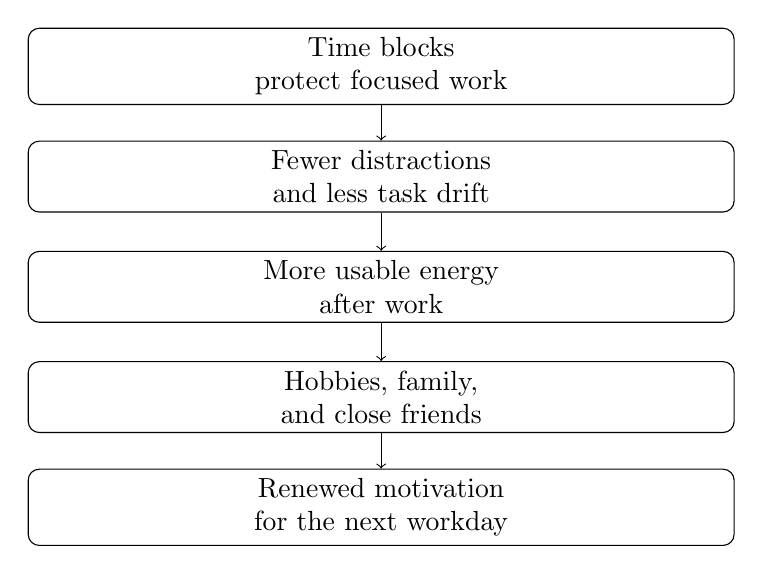
\begin{tikzpicture}
\node[draw, rounded corners, align=center, text width=0.72\linewidth] (a) at (0,0) {Time blocks\\protect focused work};
\node[draw, rounded corners, align=center, text width=0.72\linewidth] (b) at (0,-1.4) {Fewer distractions\\and less task drift};
\node[draw, rounded corners, align=center, text width=0.72\linewidth] (c) at (0,-2.8) {More usable energy\\after work};
\node[draw, rounded corners, align=center, text width=0.72\linewidth] (d) at (0,-4.2) {Hobbies, family,\\and close friends};
\node[draw, rounded corners, align=center, text width=0.72\linewidth] (e) at (0,-5.6) {Renewed motivation\\for the next workday};
\draw[->] (a) -- (b);
\draw[->] (b) -- (c);
\draw[->] (c) -- (d);
\draw[->] (d) -- (e);
\end{tikzpicture}
\caption{A transcript-derived reconstruction of the lecture's balance mechanism. No validated screenshot was preserved for this diagram.}
\end{figure}

The diagram is deliberately narrow: balance is not drawn as a sprawling life chart, but as a repeatable loop between work structure and recovery.

\section{The Practical System}

After explaining why balance matters, the speaker pivots: how do we actually become balanced? The answer comes in several practical parts, and the order matters.

\subsection{Question \& Answer}

\paragraph{Question.}
How do we move from knowing that balance matters to actually building it?

\paragraph{Answer.}
The lecture gives a system rather than a slogan: schedule the workday, protect deep work, reduce environmental interruptions, maintain hobbies outside work, and spend time with people who provide real support.

\subsection{Time Blocking}

The first practice is scheduling the day. For the speaker, the morning is the most productive period because it has the fewest distractions. That is where deep work belongs.

The workday is then divided into explicit blocks. The examples in the transcript are

\begin{equation}
T_{\mathrm{block}} \in
\{45\ \mathrm{min},\ 60\ \mathrm{min},\ 30\ \mathrm{min}\}.
\end{equation}

This gives us a simple worked example. Suppose a task needs \(30\) minutes of real focused effort. If we allocate \(60\) minutes, the unused slack is

\begin{align}
S_{60}
&=
T_{\mathrm{allocated}} - T_{\mathrm{focus}}  \\
&=
60\ \mathrm{min} - 30\ \mathrm{min} \\
&=
30\ \mathrm{min}.
\end{align}

If instead we allocate \(120\) minutes to the same task, the slack becomes

\begin{align}
S_{120}
&=
120\ \mathrm{min} - 30\ \mathrm{min} \\
&=
90\ \mathrm{min}.
\end{align}

The speaker's practical warning is that the extra slack is rarely neutral. It invites drift. In compact form,

\begin{equation}
T_{\mathrm{allocated}} \uparrow
\quad\Rightarrow\quad
S = T_{\mathrm{allocated}} - T_{\mathrm{focus}} \uparrow,
\end{equation}

provided the task itself does not really need the extra time. This is why time blocking can protect focus: it limits the container, so the work has less room to dissolve into delay.

\subsection{Environment}

The second practice is a clean desk and a good work environment. The mechanism is simple: if the tools are already near the worker, the worker does not have to keep getting up and breaking concentration.

Let \(I\) denote interruptions during a work block. The lecture's environmental claim can be stated as

\begin{equation}
\mathrm{Ready\ workspace}
\longrightarrow
I \downarrow
\longrightarrow
\mathrm{Focus} \uparrow .
\end{equation}

Again, the notation is only a careful shorthand for the spoken point. A prepared environment extends the time one can stay in the zone.

\subsection{Hobbies And Recovery}

The third practice is having hobbies or passions outside work. The speaker gives examples: going to the gym, doing something physically active, going to dinner with friends, bowling, reading in a hammock, or playing video games. The specific activity is less important than the fact that it is genuinely enjoyable and not merely passive depletion.

The mechanism is recovery. Work is easier to return to when there is something outside work that restores energy and gives the next day a reason to feel fresh.

\subsection{Family And Close Friends}

The final point is spending time with family and close friends. The speaker frames these relationships as support during the darkest moments and as the first people to celebrate wins. In entrepreneurial terms, this is part of resilience. A life organized only around output may look efficient for a while, but it removes the human support that helps a person continue through stress.

\section{Summary}

The lecture's argument is a small but serious theory of practical balance. We begin with a fixed daily budget,

\[
T_{\mathrm{day}} = 24\ \mathrm{hours},
\]

and then ask how obligations, work, self-care, relationships, and recovery can fit inside it. The speaker does not deny exceptional imbalance: entrepreneurs may work 16-hour days, and parents of newborns may lose control of their schedule. But for the ordinary majority of life, balance can be designed.

The chapter's core mechanism is this: reflection identifies stress and priorities; time blocking protects focus; a clean environment reduces interruptions; hobbies and close relationships restore energy; restored energy improves the next workday. Balance is therefore not the opposite of productivity. In this lecture, balance is one of the conditions that lets productivity continue.